\section{Question 1: Basic Image Processing and Thresholding}

In this section, image processing applications have been carried out in accordance with the tasks specified in the \texttt{EE4065 Final Project.pdf} file.

\subsection{Part A: Image Processing with Python}
The \texttt{Q1/Q1a.py} script implements the P-tile thresholding algorithm using the OpenCV library. The process consists of the following steps:
\begin{enumerate}
    \item \textbf{Image Loading:} The input image (\texttt{input.jpeg}) is read in grayscale mode.
    \item \textbf{Histogram Analysis:} The image pixel matrix is flattened into a 1D array and sorted by brightness.
    \item \textbf{Threshold Calculation (P-tile):} The algorithm identifies the brightest 1000 pixels (as specified in the project requirements) by selecting the pixel value at the $N-1000$ index from the sorted array. This value serves as the adaptive threshold.
    \item \textbf{Binarization:} A binary threshold is applied where pixels brighter than the calculated value are set to 255 (White) and others to 0 (Black).
\end{enumerate}

\subsection{Part B: Thresholding Application}
The thresholding operation is implemented on the ESP32-CAM to perform real-time processing and efficient data transmission.

\subsubsection{PC Side Implementation (\texttt{Q1/Q1b.py})}
The Python script on the PC acts as a receiver and visualization tool:
\begin{itemize}
    \item Configures a high-speed serial connection (921600 baud) to match the ESP32 transmits rate.
    \item Sends a trigger signal ('1') to request a frame.
    \item Reads exactly 76,800 bytes (320x240 resolution) from the serial buffer.
    \item Reconstructs the 1D byte array into a 2D image matrix and displays it using OpenCV.
\end{itemize}

\subsubsection{Embedded Side Implementation (\texttt{Q1/Q1b.ino})}
The firmware running on the ESP32-CAM handles image acquisition and onboard processing:
\begin{itemize}
    \item \textbf{Camera Setup:} Initializes the OV2640 sensor in grayscale mode with QVGA resolution (320x240).
    \item \textbf{Onboard Processing:} Upon receiving a request:
    \begin{enumerate}
        \item Captures a raw frame.
        \item Calculates the histogram of the image to determine pixel intensity distribution.
        \item Iterates from the brightest pixel value (255) downwards to find the threshold intensity that separates the top 1000 pixels.
        \item Modifies the frame buffer in-place: pixels above the threshold are set to 255, others to 0.
    \end{enumerate}
    \item \textbf{Transmission:} Sends the processed binary image buffer over the serial interface.
\end{itemize}

\subsection{Input and Output Data}
The input image used in the application is \texttt{Q1/Q1b\_raw.jpeg}, and the obtained thresholded output image is \texttt{Q1/Q1b\_threshold.png}.

\begin{figure}[H]
    \centering
    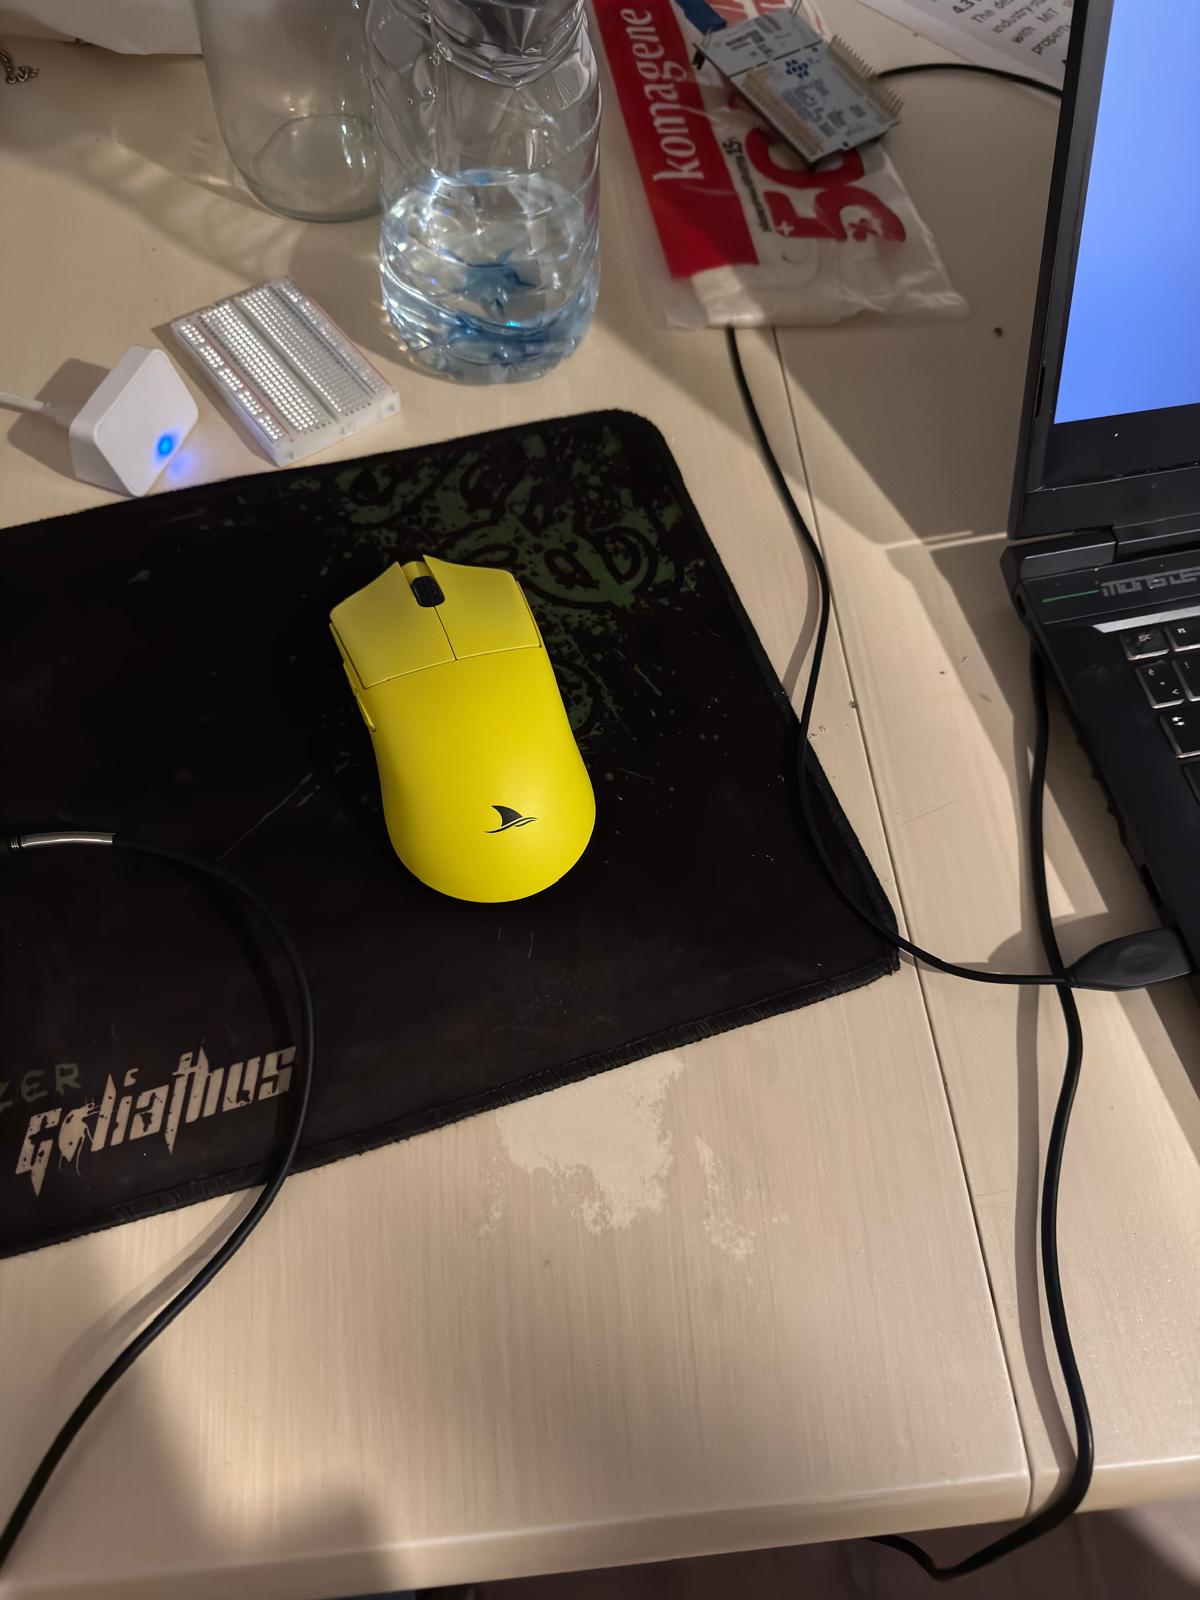
\includegraphics[width=0.6\textwidth]{../Q1/Q1b_raw.jpeg}
    \caption{Input Image (Q1b\_raw.jpeg)}
    \label{fig:q1_input}
\end{figure}

\begin{figure}[H]
    \centering
    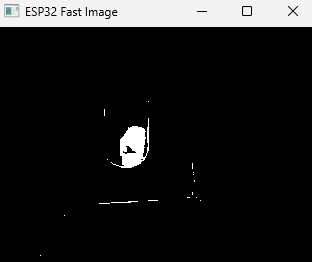
\includegraphics[width=0.6\textwidth]{../Q1/Q1b_threshold.png}
    \caption{Thresholded Output (Q1b\_threshold.png)}
    \label{fig:q1_threshold}
\end{figure}
